\documentclass{beamer}
\usepackage{listings}
\lstset{
%language=C,
frame=single, 
breaklines=true,
columns=fullflexible
}
\usepackage{blkarray}
\usepackage{subcaption}
\usepackage{url}
\usepackage{tikz}
\usepackage{tkz-euclide} % loads  TikZ and tkz-base
%\usetkzobj{all}
\usetikzlibrary{calc,math}
\usepackage{float}
\providecommand{\brak}[1]{\ensuremath{\left(#1\right)}}
\providecommand{\pr}[1]{\ensuremath{\Pr\left(#1\right)}}
\newcommand{\myvec}[1]{\ensuremath{\begin{pmatrix}#1\end{pmatrix}}}
\newcommand\norm[1]{\left\lVert#1\right\rVert}
\renewcommand{\vec}[1]{\mathbf{#1}}
\usepackage[export]{adjustbox}
\usepackage[utf8]{inputenc}
\usepackage{amsmath}
\usepackage{tikz}
\usetikzlibrary{automata, positioning}
\usetheme{Boadilla}

\title{Linear Forms Q2.18}
\author{Nelakuditi Rahul Naga - AI20BTECH11029}
\date{August 26, 2021 }
\begin{document}

\begin{frame}
\titlepage
\end{frame}

\begin{frame}
\frametitle{Question}
\begin{block}{Linear Forms Q2.18}
Find the equation of a line that cuts off equal intercepts on the coordinate axes and passes through the point $\myvec{2 \\ 3}$.
\end{block}
\end{frame}

\begin{frame}
\frametitle{Solution}
\begin{block}{General Equation of a line}
The general equation of a line can be written as :
\begin{align}
\vec{n}^T\vec{x}=c \label{eq:1}  
\end{align}
where $\vec{n}$ is the normal to the line.
\end{block}
The standard basis vectors in 2D plane are given by:
\begin{align}
\vec{e_{1}} &= \myvec{1 \\ 0}
\\\vec{e_{2}} &= \myvec{0 \\ 1}
\end{align}
\end{frame}

\begin{frame}
\frametitle{}
Let the line \eqref{eq:1} cut the x and y co-ordinate axes at $\vec{A}$ and $\vec{B}$ respectively. They can be written as :
\begin{align}
\vec{A} &= \dfrac{c\vec{e_{1}}}{\vec{n}^T\vec{e_{1}}}\label{eq:4}\\
\vec{B} &= \dfrac{c\vec{e_{2}}}{\vec{n}^T\vec{e_{2}}}\label{eq:5}
\end{align}

It is given that the line cuts off equal intercepts on the co-ordinate axes. Hence from \eqref{eq:4} and \eqref{eq:5} we have:
\begin{align}
\vec{n}^T\vec{e_{1}} = \vec{n}^T\vec{e_{2}}
\end{align}

which is equivalent to:
\begin{align}
\vec{n}^T(\vec{e_{1}}-\vec{e_{2}}) &= 0\\
\vec{n}^T\myvec{1 \\ -1} &= 0\\
\implies \vec{n} = \myvec{1 \\ 1}\label{eq:6}
\end{align}
\end{frame}

\begin{frame}{}
Hence from \eqref{eq:1} and \eqref{eq:6} , the equation of the line is given by:
\begin{align}
\myvec{1 & 1}\vec{x}=c\label{eq:7}
\end{align}
It is given that $\myvec{2 \\ 3}$ lies on the line. Hence from \eqref{eq:7} we have:
\begin{align}
c =\myvec{1 & 1}\myvec{2 \\ 3} = 5
\end{align}
Therefore the equation of the line is:
\begin{align}
\myvec{1 & 1}\vec{x}=5
\end{align}
\end{frame}

\begin{frame}
\frametitle{}
The illustration of the line is shown below :
\begin{figure}[!ht]
       \centering
    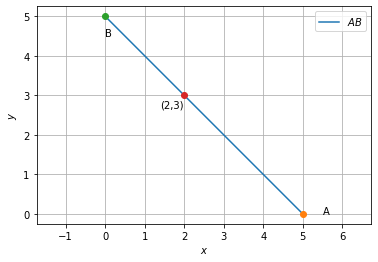
\includegraphics[width=0.8\columnwidth] {Assignment_4_Fig_1.png}
    \caption{Line $\vec{AB}$ making equal intercepts on co-ordinate axes}
    \label{Line AB}
\end{figure}
\end{frame}

\end{document}